\section{The COMPSs Programming Model}
\label{sec:compss}
COMP Superscalar \cite{compss} (and, from now on, COMPSs) is a framework aimed to ease the development of applications for distributed infrastructures. A COMPSs application is typically a normal application with some special annotations and a few extra function calls in its code.\\
\\
COMPSs applications can be written in Java, C/C++, and in Python (both 2 and 3). The Python framework is called PyCOMPSs \cite{pycompss}. All the examples and real-world usages in this project will be developed in the PyCOMPSs framework and in the Python language. However, this does not mean that all the features discussed and developed in this project are only available for PyCOMPSs. In fact, given how COMPSs is designed, the implementation of a feature for PyCOMPSs usually implies to implicitly implement it for any programming language.\\
\\
COMPSs also provides the user some tools and data that helps to monitor and to debug the applications and COMPSs itself.

\subsection{A Full Example}
\label{subsec:compss_example}
This section intends to give the reader a more or less extensive insight on what writing a PyCOMPSs application is. We think that this section may help to \textit{materialize} concepts and will avoid to give this document an excessively abstract tone.\\
\\
Lets suppose that we want to approximate the value of $\pi$. For this purpose we have thought on a simple, randomized algorithm:
\begin{enumerate}
\item Generate $N$ random points with coordinates between $-1$ and $1$
\item Consider the set of points $S$ within distance $1$ or less to the origin
\item Assume that $\frac{|S|}{N} = \frac{\pi}{4}$
\end{enumerate}

\begin{figure}[ht!]
\centering

\includegraphics[scale=0.1]{figures/circle_square.png}
\caption{A graphical representation of the random experiment. If the square has side length $2$ then the circle will have radius $1$, and therefore area $\pi$. In proportion, $\frac{\pi}{4}$ of the points belong to the circle}
\label{fig:circle_square}
\end{figure}

A more graphical explanation on why this works can be found in figure \ref{fig:circle_square}.\\
\\
We know a little bit of Python, so we have decided to implement this program in it. Basically, our small application will consist of a \verb|test_random_point| function that generates a random point and return $1$ if this point lies inside our circle, and $0$ otherwise. We will call this function $N$ times, and consider the proportion $\frac{|S|}{N}$ to be equal to $\frac{\pi}{4}$.
\newpage
\inputminted{python}{applications/PI_SQUARE/sequential.py}
Although we are happy with our $\pi$ program we notice that it is slow (figure \ref{fig:pi_size_vs_time}), and any reasonable approximation will need many experiments (figure \ref{fig:pi_size_vs_value}).\\
\\
The first thing to note is that no instance of \verb|test_random_point| depends on another one. That is, it should cause no harm to compute two or more instances of this function at the same time. If we translate it to the COMPSs language, this means that the function \verb|test_random_point| is a serious candidate to become a task. So, a first candidate of our optimized application is the following:

\inputminted{python}{applications/PI_SQUARE/pycompss_naive.py}

This example can be run with the \verb|runcompss| script.

\begin{verbatim}
runcompss -dg pycompss_naive.py 10
\end{verbatim}



\begin{figure}
\centering
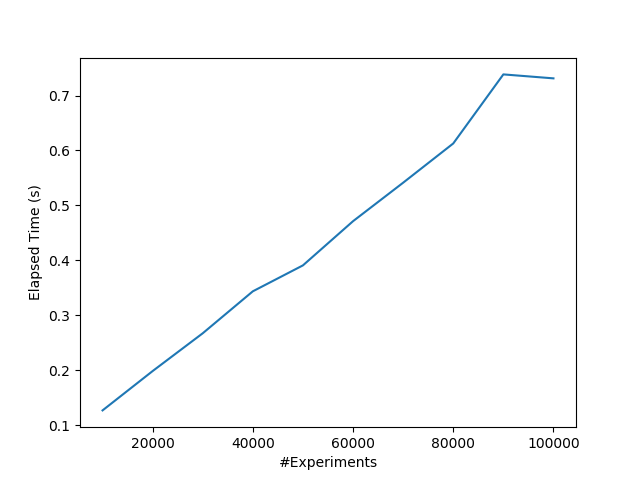
\includegraphics[scale = 0.6]{applications/PI_SQUARE/pi_size_vs_time.png}
\caption{Evolution of the necessary computation time when the number of experiments increases}
\label{fig:pi_size_vs_time}
\end{figure}

\begin{figure}
\centering
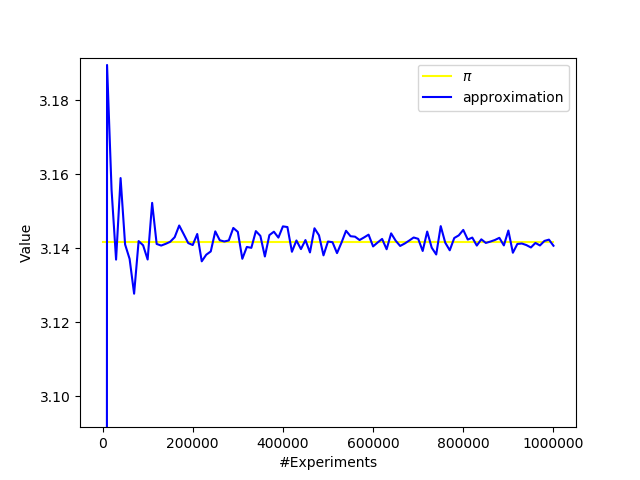
\includegraphics[scale = 0.6]{applications/PI_SQUARE/pi_size_vs_value.png}
\caption{Evolution of the obtained $\pi$ approximation when the number of experiments increases}
\label{fig:pi_size_vs_value}
\end{figure}

\subsection{COMPSs Components}
\label{subsec:compss_components}
COMPSs is designed, developed, and deployed in a modular way. This has some advantages:
\begin{itemize} 
\item Easier isolation of features
\item Partial COMPSs installations are possible (e.g: install COMPSs without PyCOMPSs)
\item Components can be individually replaced, leading to faster deployments
\end{itemize}
An overview of the main COMPSs components can be found in figure \ref{fig:compss_modules}. These components are also modularized, as seen in figures \ref{fig:runtime_modules} and \ref{fig:pycompss_modules}.
\begin{figure}
\centering
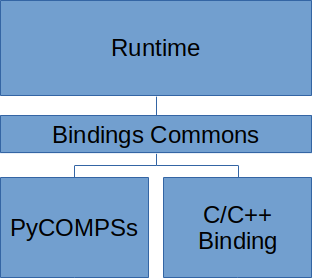
\includegraphics{figures/compss_modules.png}
\caption{Overview of the main COMPSs components. A line between two modules means that they share messages and communications between them}
\label{fig:compss_modules}
\end{figure}

%TODO: Ask Francesc help with this one
\begin{figure}
\centering

\includegraphics{figures/pending.jpg}
\caption{Overview of the main Runtime components. A line between two modules means that they share messages and communications between them}
\label{fig:runtime_modules}
\end{figure}

\begin{figure}
\centering
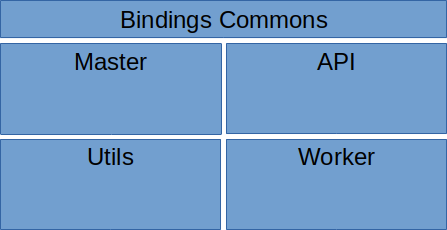
\includegraphics{figures/pycompss_modules.png}
\caption{Overview of the main PyCOMPSs components. A line between two modules means that they share messages and communications between them}
\label{fig:pycompss_modules}
\end{figure}

However, this design choice also brings some unwanted problems. The main issue is isolation and concentration of knowledge of some parts in some developers, which leads to unnecessary code replication, lack of coherence of design and implementation choices between different modules, partial feature implementations (e.g: a feature that is only available in PyCOMPSs because it was developed by someone who did not know how to implement it in the runtime), and many other things. All these issues will be adressed and referred to in this document, as they appear and play an important role in our own design choices and implementations.

%TODO
\subsection{Runtime Structure}
\label{subsec:runtime_structure}

\subsection{PyCOMPSs Structure}
\label{subsec:pycompss_structure}
PyCOMPSs can be summarized as a Python Binding for COMPSs. It gives the user a way to annotate his Python code, and it internally transforms and forwards all the derived task creation requests and data to the COMPSs Runtime. Its role can be summarized as follows:
\begin{enumerate}
\item Execute the user code, both the master and the worker part
\item Implement code annotations (\verb|@task|, \verb|@binary|, etc)
\item Implement flow control mechanisms (\verb|compss_wait_on|, \verb|compss_barrier|, etc)
\item Transform the user data into something easily to transport between different machines
\end{enumerate}


\subsection{Usability vs Performance}
\label{subsec:compss_ux_vs_perf}
COMPSs has two goals: to give the not-so-expert user an easy way to make their sequential applications run in distributed environments, and to do it as efficiently as possible. Many improvements in the COMPSs framework are aimed to improve only one of these two aspects. For example, any improvement in the communication library may improve the performance of the user application, but the user will still face the same limitations and problems when using COMPSs. Adding an automatic return completion, in case the user forgot to annotate the return value of some task, may save the user a lot of debugging time, but it will have no impact in the performance of the user application.\\
\\
COMPSs is developed and mantained by a research team in a research center, so it may be natural to think that most of the efforts and improvements are aimed to test and develop methods, models, and algorithms that improve performance, memory usage, minimize network transfers and so on. However, COMPSs is also used by other research teams as a \textit{tool} for their own purposes. Some of these teams intend to run exotic, old, complicated applications in distributed environments. Also, these teams are usually composed of researchers from fields differents than computer science, so a lack of knowledge in parallel and distributed applications should be expected. The user-oriented features intend to help these research teams, and to make their life easier in the very complicated world of distributed computing.\\
\\
This project tries to bring something that improves COMPSs in these two directions: give something to the user that makes his life easier while making COMPSs more efficient. We do not intend to limit ourselves to give the user a way to pack some parameters in a collection. We see this feature as an opportunity to give COMPSs additional intelligence that may help to improve the performance of the framework.
